\documentclass{article}
\usepackage{amsmath}
\usepackage{graphicx}
\usepackage{hyperref}
\usepackage[section]{placeins}

\hypersetup{
  colorlinks, linkcolor=red
}

\begin{document}


\title{CS838 Lab 3}
\author{Sek Cheong}
\maketitle

%\begin{abstract}
%The abstract text goes here.
%\end{abstract}

\section{Introduction}
The purpose of this project is to build a convolutional neural network (CNN) that is capable to classify images into six categories. The categories are airplane, butterfly, flower, grand  piano, starfish, and  watch. In this project we will create an CNN in Java and train it with the given training set and tuning set, and the we use the trained model to predict the images in a given test set. We will first plot the learning curve against the percentage of the train set being used, and we will the plot the learning curve against the number of epochs. 

\section{The Model}
We use the model as shown in the following illustration. The model consists of an input layer, three convolution, LuRe, Max Pool layers, and followed by a fully connected layer and a Softmax output layer with six classes. The width and height of the input layer correspond to the image width and height. The allowable image sizes are 8x8, 16x16, 32x32, 64x64, and 128x128. 

\begin{figure}[!ht]
  \centering
  \includegraphics[width=4.5in]{layers.png}
  \label{networkmodel}
  \caption{The network model}
\end{figure}


\section{The Experiment}
The first experiment is to create a learning curve that shows the accuracy verses the percentage of training sample being used. To ensure repeatability, we set the epoch to $50$ and no early stop. We start with $10\%$ of the training sample and in increment of $10\%$ in each iteration until it reaches $100\%$ of the training samples. The tuning and testing set are the full set and remain unchanged in the entire test. 

\begin{figure}[!ht]
 \centering
  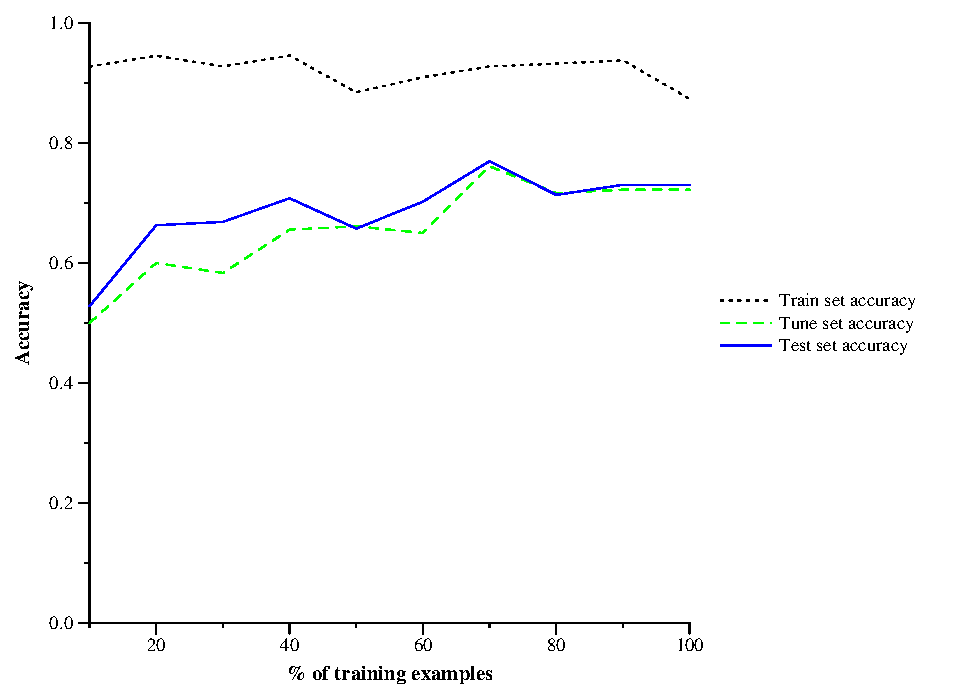
\includegraphics[width=4.8in]{size.eps}
 \label{trainsize}
 \caption{Learning curve: Accuracy vs Training set size}
\end{figure}


In the second experiment we create a learning curve that shows the accuracy verses the number of epoch the network has been trained. In this experiment we observed that the network reached its best accuracy at around $46$ epochs. The best accuracy is around $80\%$. As epoch increases the accuracy fluctuates between $70\%$ to $80\%$ then it steadily decreases to around $60\%$. 

\begin{table}[ht]
  \caption{The Confusion table}
  \centering 
  \begin{tabular}{ | l | r | r | r| r | r | r |}
    \hline
                & airplane & butterfly  & flower    &   piano  &  starfish &   watch\\ \hline
    airplane    &    38    &     0      &     1     &     0    &      0    &     2 \\ 
   butterfly    &    0     &    15      &     2     &     2    &      3    &     2 \\
      flower    &    1     &     2      &    27     &     0    &      2    &     0 \\
       piano    &    0     &     0      &     2     &    16    &      2    &     0 \\
    starfish    &    1     &     1      &     4     &     0    &      9    &     3 \\
       watch    &    1     &     0      &     1     &     1    &      1    &    39 \\
    \hline
  \end{tabular}
\end{table}

\begin{figure}[!ht]
 \centering
  \includegraphics[width=4.8in]{epoch.eps}
 \label{trainepoch}
 \caption{Learning curve: Accuracy vs Epoch}
\end{figure}

\begin{figure}[!ht]
 \centering
  \includegraphics[width=3.0in]{epoch_46_l1_filters.png}
 \label{L1filters}
 \caption{Visualization of the first convolution filters layer filters}
\end{figure}

\begin{figure}[!ht]
 \centering
  \includegraphics[width=3.0in]{epoch_46_l2_activation.png}
 \label{L1Act}
 \caption{Visualization of the first convolution layer activation}
\end{figure}


\begin{figure}[!ht]
 \centering
  \includegraphics[width=3.0in]{epoch_46_l5_filters.png}
 \label{L1filters}
 \caption{Visualization of the second convolution layer filters}
\end{figure}


\begin{figure}[!ht]
 \centering
  \includegraphics[width=3.0in]{epoch_46_l5_activation.png}
 \label{L1Act}
 \caption{Visualization of the second convolution layer activation}
\end{figure}

\section{Discussion}
From the confusion table it appears that the most hard to predict picture is star fish. The is probably due to the fact that some star fish look resemble either butterfly or flower. We tried picture of various sizes and were able to get the similar results on 16x16 images but the 8x8 images give poor results. 




\end{document}